\documentclass[10pt, letterpaper]{article}

% Packages
\usepackage[
    top=2cm,
    bottom=2cm,
    left=2cm,
    right=2cm,
    footskip=1cm
]{geometry} % Page geometry

\usepackage{titlesec} % Custom section titles
\usepackage{tabularx} % Tables with flexible width
\usepackage{array} % Additional table features
\usepackage[dvipsnames]{xcolor} % Color customization
\definecolor{primaryColor}{RGB}{0, 0, 0} % Define primary color
\usepackage{enumitem} % Customized lists
\usepackage{graphicx}

% Hyperref setup with border removed
\usepackage[
    colorlinks=true,
    urlcolor=primaryColor,
    pdfborder={0 0 0}, % Disable borders around links
    pdftitle={Dejan's CV},
    pdfauthor={Dejan Zafirev},
    pdfcreator={LaTeX}
]{hyperref}

\usepackage{bookmark} % Bookmark for PDF
\usepackage{paracol} % Multi-column layout
\usepackage{charter} % Font style

% Document Settings
\raggedright % Left-aligned text
\pagestyle{empty} % No headers/footers
\setlength{\parindent}{0pt} % No paragraph indentation
\setlength{\columnsep}{0.5cm} % Space between columns
\pagenumbering{gobble} % No page numbering

% Section style
\titleformat{\section}{\large\bfseries}{}{0pt}{}[\vspace{-1pt}\titlerule]
\titlespacing*{\section}{0pt}{0.5cm}{0.3cm} % Spacing for section titles

% Custom list bullet
\renewcommand\labelitemi{$\vcenter{\hbox{\small$\bullet$}}$}

% Custom environments
\newenvironment{highlights}{
    \begin{itemize}[topsep=3pt, leftmargin=10pt]
}{
    \end{itemize}
}

% Header environment
\newenvironment{header}{
    \centering\linespread{1.2}\vspace{0.5cm}
}{
    \vspace{0.5cm}
}

\begin{document}

% Header
\begin{header}
    \begin{tabularx}{\textwidth}{@{} X r @{}}
        % Left column: Name and Contact Information
        \begin{minipage}[b]{0.75\textwidth}
            {\fontsize{25}{25}\selectfont \textbf{Dejan Zafirev}}\\[8pt]
            Vaduz, Liechtenstein \hspace{0.5em}\textbar\hspace{0.5em}
            \href{mailto:dejan.zafirev@uni.li}{dejan.zafirev@uni.li}\\[6pt]
            \href{https://www.linkedin.com/in/dejanzafirev}{linkedin.com/in/dejanzafirev} \hspace{0.5em}\textbar\hspace{0.5em}
            \href{https://dejanzafirev.github.io}{dejanzafirev.github.io}\\[8pt]

        \end{minipage}
        &
        % Right column: Photo
        \begin{minipage}[b]{0.2\textwidth}
            \centering
            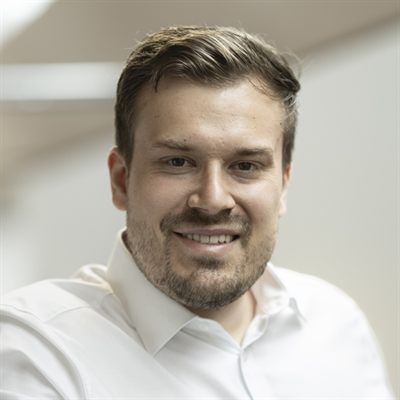
\includegraphics[width=3cm, height=3cm, keepaspectratio]{pic.jpg} % Adjust size as needed
        \end{minipage}
    \end{tabularx}
\end{header}

\vspace{-0.5cm}

% Research Interests
\section*{Research Interests}

\begin{itemize}
    \item Empirical asset pricing
    \item Political uncertainty, populism, and financial markets
    \item Derivatives, option pricing, and volatility modelling
    \item Financial econometrics and reproducible empirical methods
\end{itemize}

% Working Papers
\section*{Working Papers}

\textbf{What Drives the Price of Populism? Liberal Commitments and Market Perceptions of Political Risk} \hfill \textit{Work in progress}
\vspace{0.2cm}
\begin{itemize}
    \item Combines text-based populism and liberalism measures with option-implied risk measures to study how political uncertainty is priced in equity markets, using an event-study design around elections.
\end{itemize}

% Presentations
\section*{Presentations}

\textbf{APF International Conference of Macroeconomics and Finance} \\
\textit{Athens University of Economics and Business, Athens, Greece} \hfill \textit{July 2026}
\vspace{0.2cm}
\begin{itemize}
    \item ``What Drives the Price of Populism? Liberal Commitments and Market Perceptions of Political Risk.''
\end{itemize}

% Education
\section*{Education}

\textbf{PhD in Business Economics (Financial Economics)} \\
\textit{University of Liechtenstein, Vaduz, Liechtenstein} \hfill \textit{2025 -- Present}
\vspace{0.2cm}
\begin{itemize}
    \item Cumulative PhD thesis based on research papers in financial economics.
\end{itemize}

\vspace{0.3cm}

\textbf{MSc in Economics (Quantitative Finance Specialization)} \\
\textit{University of Freiburg, Germany} \hfill \textit{Oct 2022 -- Nov 2024}
\vspace{0.2cm}
\begin{itemize}
    \item \textbf{Key Courses:} Principles of Finance, Portfolio Management, Derivatives Pricing, Futures and Options, Industrial Organization, Intermediate Econometrics, Python Programming, Computational Economics.
    \item \textbf{Seminars:} Econometric Risk Management in Finance, Quantitative Finance (Credit Risk), Topics in Macroeconomics -- involving written reports and formal presentations.
    \item \textbf{Thesis:} ``Option Pricing Models Beyond the Black-Scholes Framework'' -- implementation of Heston, Variance Gamma, and SABR models in Python on S\&P 500 implied-volatility data, pricing Heston and Variance Gamma via the COS (Fourier-cosine) method on their characteristic functions.
    \item \textbf{Grade Average:} 1.9 (German grading system).
\end{itemize}

\vspace{0.3cm}

\textbf{BSc in Economics (Management and Finance Specialization)} \\
\textit{University of Ss. Cyril and Methodius, North Macedonia} \hfill \textit{Oct 2018 -- Jul 2022}
\vspace{0.2cm}
\begin{itemize}
    \item \textbf{Key Courses:} Financial Management, Investment Management, Econometrics, Time Series Analysis, Quantitative Methods in Finance, Financial Econometrics, Management Accounting.
    \item \textbf{Thesis:} ``Impact of Digitalization on Economic Growth'' -- panel data econometric analysis using EViews; included a cross-sectional comparison of digitalization in North Macedonia.
    \item \textbf{Grade Average:} 9.2 (Macedonian grading system).
\end{itemize}

% Professional Experience
\section*{Professional Experience}

\textbf{Research Assistant (50\%) and PhD Student} \\
\textit{University of Liechtenstein, Vaduz, Liechtenstein} \hfill \textit{July 2025 -- Present}
\vspace{0.2cm}
\begin{itemize}
    \item Conduct empirical research in financial economics, with emphasis on asset pricing, derivatives, and political uncertainty.
    \item Support research projects, reproducible empirical analysis, seminar preparation, and teaching-related activities.
\end{itemize}

\vspace{0.3cm}

\textbf{Product Control Intern} \\
\textit{HypoVereinsbank (UniCredit), Munich, Germany} \hfill \textit{Nov 2024 -- May 2025}
\vspace{0.2cm}
\begin{itemize}
    \item Analyzed daily P\&L decomposition for Equity and FICC desks, identifying unexplained drivers, and ensuring logical consistency.
    \item Collaborated with traders to resolve discrepancies and apply adjustments using internal systems and analytical tools.
    \item Delivered accurate and timely P\&L reports to senior management.
    \item Developed VBA macros to automate Excel-based workflows, improving reporting efficiency.
\end{itemize}

\vspace{0.3cm}

\textbf{Project Leader -- Erasmus+ Remote Internship} \\
\textit{CIVITTA, Estonia} \hfill \textit{Mar 2022 -- Jun 2022}
\vspace{0.2cm}
\begin{itemize}
    \item Led a student consulting team to develop a business expansion plan for an IT company entering the North Macedonian market.
    \item Coordinated tasks, ensured milestone delivery, and facilitated team communication.
    \item Built a financial model in Excel that included break-even analysis and IRR forecasts over a two-year horizon.
\end{itemize}

\vspace{0.3cm}

\textbf{Finance Intern -- Coke Summership Program} \\
\textit{Pivara Skopje (Heineken/Coca-Cola HBC)} \hfill \textit{Jul 2021 -- Aug 2021}
\vspace{0.2cm}
\begin{itemize}
    \item Supported financial operations, including contract processing and sales performance analysis.
    \item Contributed to marketing and sales initiatives by facilitating contracts and customer communication.
    \item Gained experience in time management, presentation, and cross-functional collaboration.
\end{itemize}

% Certificates
\section*{Certificates}

\textbf{Applied Data Science Lab -- WorldQuant University} \hfill \textit{Completed April 2025}
\begin{itemize}
    \item Completed project-based training in Python, SQL, data visualization, and machine learning.
    \item Built end-to-end data analysis pipelines, cleaned and analyzed real-world datasets, and developed predictive models.
    \item Final projects included portfolio risk analysis, SQL database querying, and interactive dashboards.
\end{itemize}

% Technical Skills
\section*{Technical Skills}

\begin{itemize}
    \item \textbf{Programming:} Python (Pandas, NumPy, SciPy, Matplotlib), R, SQL, LaTeX, VBA.
    \item \textbf{Tools \& Environments:} Excel, Power BI, Word, PowerPoint, PowerQuery, EViews, Jupyter Notebook, PyCharm.
\end{itemize}

% Languages
\section*{Languages}

\begin{itemize}
    \item \textbf{Macedonian:} Native
    \item \textbf{Croatian:} B1 -- Fluent
    \item \textbf{English:} C1 -- Advanced
    \item \textbf{German:} B1 -- Intermediate
\end{itemize}

\end{document}
